 \documentclass[
preprint,
nofootinbib,
amsmath,
amssymb,
aps]{revtex4-2}
%\usepackage[colorlinks=true,linkcolor=blue,urlcolor=blue,citecolor=blue,pdfusetitle]{hyperref}
\usepackage[utf8]{inputenc}
\usepackage[margin=1in,footskip=0.4in]{geometry}
\usepackage{natbib}
\usepackage{lipsum}
\usepackage[portuguese]{babel}
\usepackage{amsmath}
\usepackage[caption = false]{subfig}
\usepackage{graphicx}
\usepackage{subfig}
\usepackage{blindtext}
\usepackage{amsfonts}
\usepackage{bbm}
\usepackage{amssymb}
\usepackage{enumerate}
\usepackage{color}
\usepackage{amsthm}
\usepackage{latexsym}
\usepackage{dcolumn}
\usepackage{subfig}
\usepackage{enumitem}
\usepackage{bbold}
\usepackage{wrapfig}
\usepackage{comment}
%\renewcommand*{\bibfont}{\footnotesize}

\usepackage[compact]{titlesec}         % you need this package
\titlespacing{\section}{0pt}{0pt}{0pt} % this reduces space between (sub)sections to 0pt, for example
\AtBeginDocument{%                     % this will reduce spaces between parts (above and below) of texts within a (sub)section to 0pt, for example - like between an 'eqnarray' and text
  \setlength\abovedisplayskip{4.70pt}
  \setlength\belowdisplayskip{4.70pt}}

\usepackage{fancyhdr}% http://ctan.org/pkg/fancyhdr
\fancyhf{}
\renewcommand\footrulewidth{0.4pt}
\renewcommand\headrulewidth{0pt}



\fancyfoot[C]{\thepage}
\pagestyle{fancy}

\linespread{1.5}


%-----------Definitions----------%
\newtheorem{theorem}{Theorem}
\newtheorem{definition}{Definition}

\newcommand{\ket}[1]{\left|{#1}\right>}
\newcommand{\bra}[1]{\left<{#1}\right|}
\newcommand{\braket}[2]{\langle {#1}|{#2}\rangle}
\newcommand{\ketbra}[2]{|{#1}\rangle\langle{#2}|}
\newcommand{\Braket}[3]{\langle{#1}|{#2}|{#3}\rangle}
\newcommand{\norm}[1]{\left|\left|{#1}\right|\right|_{\text{HS}}}

\newcommand{\diff}{\mathrm{d}}
\newcommand{\Ha}{\textbf{H}}
\newcommand{\HaT}{\textbf{H}(t)}
\newcommand{\bx}{\mathbf{x}}
\newcommand{\I}{\mathbb{I}}
\newcommand{\Tr}{\mathrm{Tr}}
\newcommand{\Lx}{\mathcal{L}\left[\mathbf{q}, \dot{\mathbf{q}}\right]}
\newcommand{\Lxl}{\mathcal{L}'\left[\mathbf{1}, \dot{\mathbf{q}}\right]}
\newcommand{\Hx}{\mathcal{H}'\left[\mathbf{q}, \dot{\mathbf{p}}\right]}
\newcommand{\vx}{v_{\text{adb}}\left[\mathbf{x}, \dot{\mathbf{x}}\right]}
\newcommand{\tn}{\textnormal{t}}




\begin{document}


\begin{titlepage}
\thispagestyle{empty}
\begin{center}
\begin{minipage}{0.75\linewidth}
    \centering
	 {\large Universidade Federal de São Carlos\par}
	 {\large Programa de Pós-graduação em Física/CCET\par}

	\par
    \vspace{1.5cm}
%Thesis title
    {\bf{\uppercase{\large  Introdução a computação quântica, algoritmos quânticos teoria e prática.
    \par}}}
    \vspace{3cm}

%Author's name
    {\large Autor: Gubio Gomes de Lima
 \par}
    \vspace{3cm}
%Degree
    {\large Fundamentos para construir seu "computador quântico"\par}
    \vspace{4cm}
%Date
    {\large {\today}}

\end{minipage}
\end{center}
\end{titlepage}
\setcounter{page}{0}

%\pdfbookmark

\tableofcontents
\newpage


%\textbf{Faltou índice!!!}
\newpage
\section{Introdução}

Os computadores quânticos são uma tecnologia emergente com um potencial incrível para resolver problemas intratáveis até mesmo para os maiores supercomputadores atuais. 
\newpage
\section{Introdução à computação clássica.}
Nesse capítulo, você irá aprender os conceitos fundamentais da computação quântica e clássica. Antes de nos aprofundarmos na computação quântica, precisamos de um arcabouço para descrever os qubits e as operações que podemos realizar sobre eles. Para em seguida criar do zero seus primeiros qubits e algoritmos de uma forma prática utilizando NumPy (Numba), PyTorch e Jax. 

 O que você irá aprender:
\begin{itemize}
    \item Entender o que é um Bit e Qubit, como criar, descrever, manipular, representar.
    \item Definir e fornecer exemplos de um sistema quântico em uma superposição e como criar.
    
    \item Declarar a relação entre amplitudes e probabilidades de resultados de medições, e explicar o que significa um estado ser normalizado.
    \item Explicar como operações são aplicadas matematicamente a estados de qubits.
\end{itemize}
 
\newpage
\subsection{A menor unidade de informação: Bit.}
Nesta seção, buscamos responder às seguintes perguntas: 
\begin{center}
    \textit{O que são bits e como os computadores os criam?}
\end{center}
Computadores convencionais, também chamados de computadores clássicos, representam informações por meio de bits. Mas o que é essa informação? Ela pode assumir diversas formas, como imagens, dados de um scanner, impressões digitais, sons ou textos. No entanto, todas essas informações, independentemente de sua natureza, são convertidas em números ou caracteres, que, por sua vez, são transformados em bits. Esses bits consistem em uma sequência de números binários, cada um podendo assumir o valor 0 ou 1. Na tabela a seguir temos 4 exemplos para as letras “a” e "b" e os números $1$ e $2$ : 
\begin{table}[h!]
    \centering
    \begin{tabular}{|c|c|c|}
        \hline
        \textbf{Caractere} & \textbf{Decimal (ASCII)}  & \textbf{Representação em Bits.} \\ \hline
        a & 97 & 01100001 \\ \hline
        b & 98 & 01100010 \\ \hline
        1 & 49 & 00110001 \\ \hline
        2 & 50 & 00110010 \\ \hline
    \end{tabular}
    \caption{Tabela com caracteres e suas representações em valor ASCII (\textit{American Standard Code for Information Interchange}) em binário.}
    \label{tab:caracteres_bits}
\end{table}

O leitor pode estar se perguntando, “como converter caracteres para binário?". 
A conversão de caracteres para binário utilizando a tabela ASCII envolve dois passos principais: identificar o valor decimal correspondente e convertê-lo para binário. Cada caractere possui um código numérico na tabela ASCII, então o primeiro passo é identificar qual o valor decimal do caractere que você quer converter. Por exemplo, a letra \textbf{a} tem valor decimal $97$ e o número $1$ tem valor decimal $49$. O segundo, converter o valor decimal para binário. A conversão para binário pode ser feita dividindo o número decimal sucessivamente por 2, anotando os restos até chegar a zero. Mostraremos isso com exemplos:

\subsubsection*{Exemplo 1: Converter a letra \textbf{a}}
\begin{enumerate}
    \item O código ASCII de \textbf{a} é \textbf{97}.
    \item Dividindo sucessivamente por 2:
    \begin{align*}
        97 \div 2 &= 48 \text{, resto } 1 \\
        48 \div 2 &= 24 \text{, resto } 0 \\
        24 \div 2 &= 12 \text{, resto } 0 \\
        12 \div 2 &= 6 \text{, resto } 0 \\
        6 \div 2 &= 3 \text{, resto } 0 \\
        3 \div 2 &= 1 \text{, resto } 1 \\
        1 \div 2 &= 0 \text{, resto } 1
    \end{align*}
    \item Lendo os restos de baixo para cima: \textbf{01100001}.
\end{enumerate}
Portanto, a letra \textbf{a} em binário é \textbf{01100001}.

\subsubsection*{Exemplo 2: Converter o número \textbf{1}}
\begin{enumerate}
    \item O código ASCII de \textbf{1} é \textbf{49}.
    \item Dividindo sucessivamente por 2:
    \begin{align*}
        49 \div 2 &= 24 \text{, resto } 1 \\
        24 \div 2 &= 12 \text{, resto } 0 \\
        12 \div 2 &= 6 \text{, resto } 0 \\
        6 \div 2 &= 3 \text{, resto } 0 \\
        3 \div 2 &= 1 \text{, resto } 1 \\
        1 \div 2 &= 0 \text{, resto } 1
    \end{align*}
    \item Lendo os restos de baixo para cima: \textbf{00110001}.
\end{enumerate}
Portanto, o número \textbf{1} em binário é \textbf{00110001}\footnote{ Nota: A codificação ASCII utiliza 8 bits para representar cada caractere. Quando o binário resultante possui menos de 8 dígitos, adicionamos zeros à esquerda para completar o padrão. Por isso, o valor \textbf{1100001} torna-se \textbf{01100001}}.

VER ESSA REFERENCIA SOBRE OPERAÇOES CLASSICA DE SOMA MULTIPLICAÇAO COM XOR OR ... :

https://www.makerhero.com/blog/o-que-sao-portas-logicas/?srsltid=AfmBOoodmfMRcMQi3X55XNxUUZQLrTjqgVngCicpLpeuxwAnJp1eJ3mZ
\section*{Exercício Proposto.}
Agora que você aprendeu a converter caracteres para binário, siga os passos descritos no tutorial para realizar as conversões dos seguintes exercícios:

\begin{itemize}
    \item Converta a letra \textbf{b}.
    \item Converta o número \textbf{2}.
\end{itemize}

Para entender como os bits são criados, voltaremos um pouco na história dos computadores. O \textbf{Electronic Numerical Integrator and Computer (ENIAC)} foi um dos primeiros computadores totalmente eletrônicos e digitais de grande escala. Desenvolvido pelos cientistas norte-americanos John Eckert e John Mauchly, o ENIAC começou a operar em fevereiro de 1946. Ele foi projetado para realizar cálculos numéricos complexos, inicialmente voltados para aplicações militares, como o cálculo de trajetórias balísticas. Seu design inovador utilizava cerca de 18.000 válvulas termiônicas (também chamadas de tubos de vácuo), que funcionavam como chaves para representar os estados $0$ e $1$. % Então, para  criar o bit, é sempre necessário associar a algo físico, que pode estar em dois estados diferentes. 

{\color{red} Quantos tempo leva para fazer um cálculo?}

{\color{red} Isso é um tipo de computação analógica?}

{\color{red} Qual o tamanho do dispositivo?}

{\color{red} Qual o tempo para executar um código/protocolo/atividade?}

O ENIAC era programado manualmente por meio da conexão de cabos e da configuração de interruptores. Apesar de sua grande capacidade para a época, era muito trabalhoso reconfigurá-lo para diferentes cálculos, pois isso exigia mudanças físicas nos cabos e chaves. Por outro lado, antes do ENIAC, o \textbf{Mark I}, desenvolvido na Universidade de Harvard, é frequentemente citado como o primeiro computador. No entanto, ele era um dispositivo \textit{eletromecânico}, e não totalmente eletrônico. Isso significa que o Mark I utilizava componentes mecânicos, como relés, combinados com circuitos elétricos para processar dados. Sua operação era consideravelmente mais lenta do que a do ENIAC, devido ao tempo necessário para movimentar as partes mecânicas.

{\color{red} Figura que represente o texto}

Enquanto o Mark I dependia de componentes mecânicos para alternar entre os estados \(0\) e \(1\), o ENIAC representava uma grande evolução ao utilizar válvulas termiônicas, que permitiam transições muito mais rápidas e aumentaram significativamente a velocidade de processamento. Essa mudança marcou o início da era dos computadores eletrônicos. Assim, o ENIAC foi o primeiro computador digital e eletrônico de grande escala, demonstrando o potencial dos sistemas binários na computação e abrindo caminho para o desenvolvimento dos computadores modernos.

Nos computadores modernos, os bits são representados por níveis de tensão elétrica em circuitos integrados. O estado \(0\) representa um nível de tensão mais baixo, que pode ser próximo a \(0\) Volts (V), e o estado \(1\) representa um nível de tensão mais alto, que depende do padrão do circuito. Em processadores modernos da \textbf{AMD} e \textbf{Intel}, a tensão de operação pode variar entre \(0,7\) V a \(1,2\) V para um estado \(1\), enquanto o estado \(0\) é próximo de \(0\) V. A corrente, por sua vez, pode variar dependendo da carga que o circuito está processando, mas, em geral, os processadores modernos operam com correntes muito baixas, na ordem de miliampères (mA), devido ao design eficiente e ao uso de tecnologia de transistores de baixa potência.

Para gerar e controlar os estados binários, os computadores modernos utilizam dispositivos feitos de \textit{semicondutores}, como os \textbf{transistores}. Transistores são dispositivos eletrônicos que funcionam como interruptores, com dois estados possíveis: \textit{ligado} (conduzindo corrente elétrica) e \textit{desligado} (não conduzindo corrente elétrica). Eles são os componentes fundamentais nos circuitos lógicos de qualquer processador. Podemos pensar nos transistores como "nano-interruptores eletrônicos". Eles são extremamente pequenos e rápidos, permitindo a operação de bilhões de transistores em um único chip de computador. Um transistor funciona de maneira semelhante a um interruptor convencional: quando está ligado, permite que a corrente flua, representando o estado $1$; quando está desligado, a corrente não flui, representando o estado $0$.

\begin{figure}
    \centering
    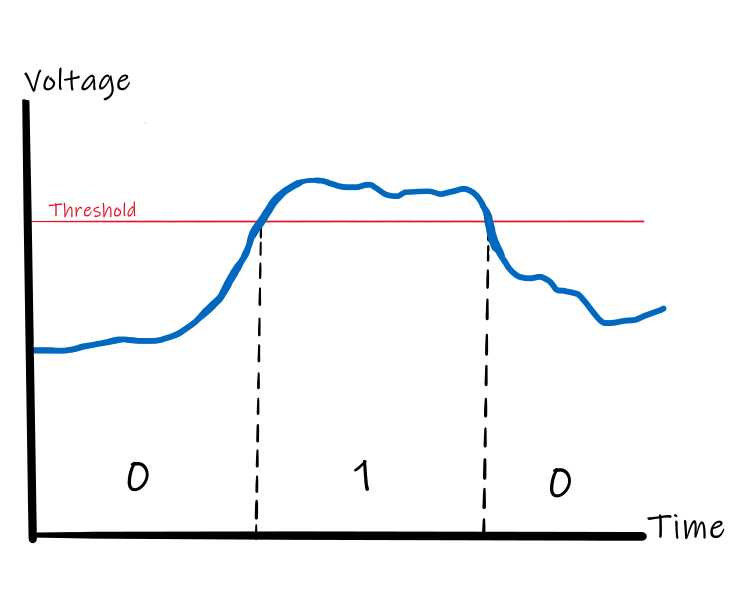
\includegraphics[width=0.5\linewidth]{img/voltage_threshold.png}
    \caption{ Uma tensão elétrica passando por um componente eletrônico usado para representar bits. O threshold é um valor limite para o qual a tensão é associada a um bit no estado 1, e qualquer valor abaixo para um bit no estado 0.}
    \label{fig:enter-label}
\end{figure}

Esses transistores são organizados em \textit{circuitos lógicos} que processam as operações computacionais. Em termos simples, esses circuitos lógicos realizam operações como \textit{E}, \textit{OU}, \textit{NÃO}, combinadas para formar instruções mais complexas. A eficiência e a velocidade dos computadores modernos são na maioria atribuídas ao avanço na miniaturização dos transistores, o que permite que um número maior de operações sejam realizadas por segundo. A velocidade de execução dos computadores modernos é incrivelmente alta devido à miniaturização dos transistores. Processadores atuais, como os da AMD e Intel, podem ter bilhões de transistores em um único chip, com cada transistor ligando e desligando em frações de segundo. A velocidade de comutação dos transistores modernos é da ordem de \textit{gigaherços (GHz)}, ou seja, bilhões de ciclos por segundo.

{\color{red}
Qual o tamanho do dispositivo?}

{\color{red} Qual o tempo para executar um código/protocolo/atividade?}


{\color{red} Qual foi a evolução?}


Comparando com os primeiros computadores, como o ENIAC, a diferença é abismal. O ENIAC tinha componentes como válvulas termiônicas que eram muito mais lentos do que os transistores atuais, além de consumir muito mais energia. Já os transistores modernos, com seu tamanho reduzido para a escala de nanômetros (\(nm\)), operam de forma muito mais eficiente e rápida. Em processadores atuais, o tamanho de um transistor pode ser tão pequeno quanto \(7\) nm, enquanto no ENIAC, os componentes eram muito maiores, e a velocidade de processamento era limitada.


Outro passo importante é como os bits são lidos e interpretados pelos computadores. Para isso, é fundamental compreender o processo de conversão \textit{Analógico-Digital} (A/D). Muitos dispositivos reais, como sensores e microfones, geram sinais \textit{analógicos}, que são contínuos e podem assumir uma infinidade de valores. Por exemplo, um sensor de temperatura pode gerar um valor de tensão que varia continuamente de $0$ a $5$ Volts à medida que a temperatura muda.

No entanto, os computadores trabalham apenas com dados \textit{digitais}, ou seja, dados representados por uma sequência de $0$s e $1$s. Para um sinal analógico ser processado por um computador, ele precisa ser convertido para um formato digital. Isso é feito por dispositivos chamados \textbf{Conversores Analógico-Digital (ADC, do inglês \textit{Analog-to-Digital Converter})}.

Um ADC recebe um sinal analógico e o converte para um valor digital representado por uma sequência de bits. Esse processo ocorre em duas etapas principais:
\begin{enumerate}
    \item \textbf{Amostragem}: O sinal analógico é amostrado em intervalos regulares de tempo. A cada amostra, o valor do sinal analógico é medido.
    \item \textbf{Quantização}: O valor medido da amostra é então arredondado para o valor binário mais próximo, representando a tensão naquele ponto. Quanto maior a resolução do ADC (ou seja, maior o número de bits), mais precisa será a representação do valor analógico.
\end{enumerate}

Por exemplo, se tivermos um sinal analógico variando entre $0$ a $5$ Volts e um ADC de 3 bits, ele poderá representar $8$ valores discretos (de $000$ a $111$) que corresponderiam a diferentes intervalos de tensão. Se o sinal analógico for, por exemplo, $2,5$ Volts, o ADC atribuiria a ele o valor binário $010$, que é o valor mais próximo da tensão medida, na resolução disponível.

Essa conversão analógico-digital permite que dispositivos reais, como sensores de temperatura, pressão, ou até mesmo sinais de áudio, sejam lidos, processados e armazenados pelos computadores, que só conseguem entender valores binários. Assim, a conversão A/D é essencial para integrar o mundo analógico com a computação digital, possibilitando que o computador interaja com o ambiente físico de maneira eficiente.

{\color{red} Problemas e dificuldades da computação clássica. Comentar sobre erros nesses processos}

%Sugestão: Pedir para amandar corrigir a seção bit classico, e adicionar essa parte.



%#####################
\newpage


\newpage
\section{Introdução a computação quântica.}

Nesta seção, buscamos responder às seguintes perguntas: 
\begin{center}
    \textit{O que são qubits e como os computadores quânticos os criam?}
\end{center}
para responder essa perguntar iremos ...

O poder dos computadores quânticos advém da maneira distinta como eles representam e manipulam informações. Computadores quânticos utilizam bits especiais, chamados de bits quânticos, ou qubits. Assim como os bits clássicos, os qubits também correspondem a algo físico. Nosso foco no momento será nos conceitos essenciais da teoria com perspectiva de desenvolvimento de software e algoritmos.
Nos dedicaremos no capítulo  7 sobre o desenvolvimento físico dos qubits.



\subsection{Bit quântico.}


\subsection*{Representação matemática do estado de um qubit.}

\subsection{Normalização dos estados.}

\subsection{Produto interno e base ortogonal.}

\subsection{Superposição.}

\subsection{Probabilidade de resultado de medição.}

\subsection*{Amostragem nas medidas.}

\subsection{Operações em estados de um qubits.}

\subsection*{Aplicando uma operação quântica.}

\subsection{Simples algoritmo quântico.}
% \begin{itemize}
%     \item Um meio de medir um qubit para determinar em que estado ele se encontra;
%     \item Uma forma de manipular o estado de um qubit para realizar cálculos.
% \end{itemize}



\newpage
\section{Hand on: construindo seu computação quantica }
\newpage
\section{Algoritmos basicos}



\newpage
\section{Algoritmos variacionais}
\newpage
\section{Plataformas de computação quântica }

\subsection{Supercondutor}
\subsection{Átomos neutros}
\subsection{Fotonico }
\subsection{Outro }
\newpage
\section{Aprofundamento das skills.}
Cada subseção complementa uma skill do site Quantum Learning com um resultado demonstrado ou um passo além do curso. A referência de estrutura é T. G. Wong, \textit{Introduction to Classical and Quantum Computing}; o texto é original.

% ---------- Fundamentos Básicos ----------
\subsection{Bits e números binários.}
Todo inteiro $N$ com $0 \le N < 2^n$ tem uma única representação com $n$ bits. Existem $2^n$ sequências e $2^n$ inteiros nesse intervalo, então basta mostrar que sequências diferentes dão números diferentes. Se $b$ e $b'$ diferem e $k$ é a posição mais alta em que diferem, as posições abaixo de $k$ contribuem com no máximo
\begin{equation}
    \sum_{j=0}^{k-1} 2^j = 2^k - 1 < 2^k,
\end{equation}
o que não compensa a diferença $2^k$. Logo os números são distintos. Em consequência, para representar $M$ possibilidades são necessários $\lceil \log_2 M \rceil$ bits.

\subsection{Portas lógicas clássicas.}
Toda função $f:\{0,1\}^n \to \{0,1\}$ pode ser escrita com NOT, AND e OR. Para cada entrada $a$ com $f(a)=1$, forme o produto $m_a(x)$ das variáveis, negando $x_i$ quando $a_i = 0$. Esse produto vale $1$ apenas em $x=a$, e portanto
\begin{equation}
    f(x) = \sum_{a:\,f(a)=1} m_a(x),
\end{equation}
em que a soma é o OR. É a forma normal disjuntiva. Como NOT, AND e OR se constroem com NAND, a NAND é universal.

\subsection{Codificando informação com ASCII.}
A UTF-8 estende o ASCII sem ambiguidade. Um byte que começa com $0$ é um caractere ASCII; um caractere longo começa com um byte $110\ldots$, $1110\ldots$ ou $11110\ldots$, que indica 2, 3 ou 4 bytes, e todos os bytes seguintes começam com $10$. Como nenhum byte inicial começa com $10$, um leitor que entra no meio do texto encontra o início do próximo caractere. Um caractere de 2 bytes tem $5 + 6 = 11$ bits livres.

\subsection{Portas reversíveis.}
Apagar informação tem um custo físico mínimo. Pelo princípio de Landauer, apagar um bit num ambiente à temperatura $T$ dissipa pelo menos
\begin{equation}
    E = k_B T \ln 2,
\end{equation}
cerca de $2{,}9\times 10^{-21}\,$J a $300\,$K. Uma computação reversível não apaga bits e, em princípio, escapa desse limite. Para qualquer $f$, a função $(x, y) \mapsto (x, y \oplus f(x))$ é reversível, pois é a própria inversa: $y \oplus f(x) \oplus f(x) = y$. É essa forma que os oráculos quânticos usam.

\subsection{O qubit e a superposição.}
Um qubit tem dois graus de liberdade reais. As amplitudes $\alpha$ e $\beta$ somam quatro números reais; a normalização retira um, e a fase global, outro. Escolhendo a fase de modo que $\alpha \ge 0$,
\begin{equation}
    \ket{\psi} = \cos\frac{\theta}{2}\ket{0} + e^{i\phi}\sin\frac{\theta}{2}\ket{1}, \qquad 0\le\theta\le\pi,\; 0\le\phi<2\pi.
\end{equation}

\subsection{Medida quântica.}
As coordenadas do estado acima na esfera de Bloch são valores esperados das matrizes de Pauli:
\begin{equation}
    x = \Braket{\psi}{X}{\psi} = \sin\theta\cos\phi, \quad y = \Braket{\psi}{Y}{\psi} = \sin\theta\sin\phi, \quad z = \Braket{\psi}{Z}{\psi} = \cos\theta.
\end{equation}
Vale $x^2+y^2+z^2=1$ e $P(0) = (1+z)/2$. Com $N$ repetições, a estimativa de $p = P(0)$ tem desvio padrão $\sqrt{p(1-p)/N}$: para reduzir o erro à metade, é preciso quadruplicar o número de medidas.

\subsection{Portas de 1 qubit.}
Como $X^2 = I$, a série da exponencial se separa em potências pares e ímpares, e o mesmo vale para $Y$ e $Z$. As rotações são
\begin{equation}
    R_x(\theta) = e^{-i\theta X/2} = \cos\frac{\theta}{2}\, I - i\sin\frac{\theta}{2}\, X.
\end{equation}
Em particular, $R_x(\pi) = -iX$: a porta X é um giro de $\pi$ em torno do eixo $x$, a menos de fase global. Toda porta de 1 qubit se escreve como $e^{i\delta}R_z(a)R_y(b)R_z(c)$.

\subsection{Introdução a circuitos quânticos.}
A identidade $HZH = X$ se verifica por multiplicação direta:
\begin{equation}
    HZH = \frac12 \begin{pmatrix} 1 & 1 \\ 1 & -1 \end{pmatrix}\begin{pmatrix} 1 & 1 \\ -1 & 1 \end{pmatrix} = \begin{pmatrix} 0 & 1 \\ 1 & 0 \end{pmatrix} = X,
\end{equation}
em que usamos $ZH = \frac{1}{\sqrt2}\begin{pmatrix} 1 & 1 \\ -1 & 1 \end{pmatrix}$. Trocando Z por um giro $R_z(\phi)$ entre as duas portas H, obtemos $P(0) = \cos^2(\phi/2)$: a fase, invisível na medida direta, vira probabilidade. É o interferômetro mais simples.

% ---------- Álgebra Linear ----------
\subsection{Vetores coluna e linha.}
O conjugado transposto de um produto inverte a ordem, $(AB)^\dagger = B^\dagger A^\dagger$. De fato,
\begin{equation}
    \left[(AB)^\dagger\right]_{ij} = \Big(\sum_k A_{jk}B_{ki}\Big)^* = \sum_k (B^\dagger)_{ik}(A^\dagger)_{kj}.
\end{equation}
Para um ket transformado, $\ket{\psi'} = U\ket{\psi}$ implica $\bra{\psi'} = \bra{\psi}U^\dagger$.

\subsection{Produto interno e ortonormalidade.}
Vale a desigualdade de Cauchy--Schwarz, $|\braket{\phi}{\psi}|^2 \le \braket{\phi}{\phi}\braket{\psi}{\psi}$. Para estados normalizados, tome $\ket{\chi} = \ket{\psi} - \braket{\phi}{\psi}\ket{\phi}$. Então
\begin{equation}
    0 \le \braket{\chi}{\chi} = 1 - |\braket{\phi}{\psi}|^2.
\end{equation}
Isso garante que $|\braket{\phi}{\psi}|^2$ pode ser interpretado como probabilidade.

\subsection{Projeções e mudança de base.}
Dada uma lista de vetores linearmente independentes, o processo de Gram--Schmidt produz uma base ortonormal subtraindo projeções:
\begin{equation}
    \ket{u_k} = \ket{v_k} - \sum_{j<k} \ket{e_j}\braket{e_j}{v_k}, \qquad \ket{e_k} = \frac{\ket{u_k}}{\sqrt{\braket{u_k}{u_k}}}.
\end{equation}
A matriz que muda da base $\{\ket{e_j}\}$ para $\{\ket{f_i}\}$ tem elementos $\braket{f_i}{e_j}$ e é unitária.

\subsection{Portas quânticas como matrizes unitárias.}
Toda matriz que preserva a norma de todos os vetores é unitária. Seja $M = U^\dagger U - I$, que é hermitiana. Se $\Braket{\psi}{M}{\psi}=0$ para todo $\ket{\psi}$, em particular isso vale para os autovetores de $M$, e então todos os seus autovalores são nulos. Como $M$ é diagonalizável, $M=0$. Portanto a unitariedade é consequência de exigir linearidade e probabilidade total igual a 1.

\subsection{Produto externo e completude.}
Um operador fica determinado por seus elementos de matriz. Inserindo a completude dos dois lados,
\begin{equation}
    A = \Big(\sum_i \ketbra{e_i}{e_i}\Big) A \Big(\sum_j \ketbra{e_j}{e_j}\Big) = \sum_{ij} \Braket{e_i}{A}{e_j}\,\ketbra{e_i}{e_j}.
\end{equation}
O traço independe da base e vale $\Tr(\ketbra{\psi}{\phi}) = \braket{\phi}{\psi}$.

\subsection{Circuitos quânticos e unitariedade.}
Autovetores de uma unitária com autovalores distintos são ortogonais. Se $U\ket{v}=\lambda\ket{v}$ e $U\ket{w}=\mu\ket{w}$, com $|\lambda|=|\mu|=1$, então
\begin{equation}
    \braket{v}{w} = \Braket{v}{U^\dagger U}{w} = \lambda^*\mu\,\braket{v}{w}.
\end{equation}
Se $\lambda\ne\mu$, então $\lambda^*\mu \neq 1$ e $\braket{v}{w}=0$. Assim, toda unitária se escreve como $\sum_k e^{i\theta_k}\ketbra{v_k}{v_k}$.

% ---------- Computação Quântica ----------
\subsection{Produto tensorial.}
A regra $(A\otimes B)(C\otimes D) = AC\otimes BD$ mostra que portas em qubits diferentes comutam:
\begin{equation}
    (A\otimes I)(I\otimes B) = A\otimes B = (I\otimes B)(A\otimes I).
\end{equation}
Para $n$ qubits, aplicar H em todos leva $\ket{0\cdots0}$ à superposição uniforme $2^{-n/2}\sum_x \ket{x}$, ponto de partida de muitos algoritmos.

\subsection{Medindo vários qubits.}
A medida do primeiro qubit é descrita pelos projetores $\Pi_m = \ketbra{m}{m}\otimes I$:
\begin{equation}
    P(m) = \Braket{\psi}{\Pi_m}{\psi}, \qquad \ket{\psi_m} = \frac{\Pi_m\ket{\psi}}{\sqrt{P(m)}}.
\end{equation}
Como os $\Pi_m$ e os projetores do segundo qubit comutam, a distribuição conjunta não depende da ordem das medidas.

\subsection{Estados emaranhados e estados produto.}
Organize as amplitudes na matriz $C = (c_{ij})$. O estado é produto se e só se $C$ tem posto 1, isto é, $\det C = 0$ para dois qubits. Pela decomposição em valores singulares existem bases em que
\begin{equation}
    \ket{\psi} = s_1\ket{e_1}\ket{f_1} + s_2\ket{e_2}\ket{f_2}, \qquad s_1^2+s_2^2=1,
\end{equation}
a decomposição de Schmidt. Como portas locais multiplicam $C$ por unitárias, elas não alteram $s_1$ e $s_2$. A concorrência vale $2|\det C| = 2 s_1 s_2$.

\subsection{Portas de 2 qubits: CNOT e Toffoli.}
Na base X, a CNOT troca os papéis de controle e alvo:
\begin{equation}
    \text{CNOT}\ket{+}\ket{-} = \frac{1}{\sqrt2}\big(\ket{0}\ket{-} - \ket{1}\ket{-}\big) = \ket{-}\ket{-}.
\end{equation}
O alvo está num autovetor de X com autovalor $-1$, e o sinal passa para o controle. Esse efeito, o \textit{phase kickback}, é o mecanismo dos algoritmos de Deutsch--Jozsa, Bernstein--Vazirani e da estimação de fase.

\subsection{Teorema da não-clonagem.}
Copiar com perfeição permitiria distinguir estados não ortogonais, e por isso viola a unitariedade. Cópias imperfeitas, porém, existem: a melhor copiadora universal de um qubit para dois (Bu\v{z}ek e Hillery) produz cópias com fidelidade
\begin{equation}
    F = \frac56,
\end{equation}
igual para todos os estados de entrada.

\subsection{Conjuntos universais de portas.}
A porta T não pertence ao grupo de Clifford porque não leva matrizes de Pauli em matrizes de Pauli:
\begin{equation}
    T X T^\dagger = \frac{X + Y}{\sqrt2}.
\end{equation}
Já $S X S^\dagger = Y$ e $H X H = Z$. O teorema de Gottesman--Knill se apoia nisso: um circuito de Clifford é simulado acompanhando apenas $n$ produtos de Pauli que estabilizam o estado.

% ---------- Teoria Quântica ----------
\subsection{Estados de Bell.}
Cada qubit de um par de Bell, visto isoladamente, está no estado maximamente misto. Com $\rho = \ketbra{\Phi^+}{\Phi^+}$, o traço parcial sobre o segundo qubit dá
\begin{equation}
    \rho_1 = \Tr_2\,\rho = \frac12\big(\ketbra{0}{0} + \ketbra{1}{1}\big) = \frac{I}{2}.
\end{equation}
O par como um todo é conhecido por completo, e cada parte é totalmente aleatória: isso não tem análogo clássico.

\subsection{Desigualdade CHSH.}
Sejam $A_x$ e $B_y$ observáveis com autovalores $\pm1$, os de Alice comutando com os de Bob, e
\begin{equation}
    \mathcal{S} = A_0B_0 + A_0B_1 + A_1B_0 - A_1B_1.
\end{equation}
Usando $A_x^2=B_y^2=I$, obtemos $\mathcal{S}^2 = 4I - [A_0,A_1][B_0,B_1]$. Cada comutador tem norma no máximo 2, então $\mathcal{S}^2 \le 8$ e $|\langle\mathcal{S}\rangle|\le 2\sqrt2$, o limite de Tsirelson. No caso clássico os comutadores são nulos e resta $|S|\le2$. A probabilidade de vitória no jogo é $\frac12 + \frac{S}{8}$.

\subsection{Codificação superdensa.}
O emaranhamento compartilhado é indispensável. Pelo teorema de Holevo, $n$ qubits enviados sem emaranhamento prévio transmitem no máximo $n$ bits. Com um par $\ket{\Phi^+}$, os quatro estados $(\sigma\otimes I)\ket{\Phi^+}$, com $\sigma\in\{I,X,Z,ZX\}$, são ortogonais, pois
\begin{equation}
    \Braket{\Phi^+}{\sigma^\dagger\tau\otimes I}{\Phi^+} = \frac12\Tr(\sigma^\dagger\tau).
\end{equation}

\subsection{Teletransporte quântico.}
A identidade central se obtém expandindo os dois primeiros qubits na base de Bell:
\begin{equation}
    \ket{\psi}\ket{\Phi^+} = \frac12\Big[\ket{\Phi^+}\ket{\psi} + \ket{\Phi^-}Z\ket{\psi} + \ket{\Psi^+}X\ket{\psi} + \ket{\Psi^-}XZ\ket{\psi}\Big].
\end{equation}
Antes de receber os bits, o estado de Bob é a média dos quatro casos, $\frac14\sum_\sigma \sigma\ketbra{\psi}{\psi}\sigma^\dagger = I/2$, que não depende de $\ket{\psi}$: nenhuma informação chega sem o canal clássico.

\subsection{Distribuição de chaves: BB84.}
Seja $Q$ a taxa de erro medida nos bits peneirados. Com correção de erros e amplificação de privacidade ideais, a fração de chave secreta por bit peneirado é
\begin{equation}
    r = 1 - 2h(Q), \qquad h(Q) = -Q\log_2 Q - (1-Q)\log_2(1-Q).
\end{equation}
A taxa $r$ se anula em $Q \approx 11\%$. O ataque de interceptar e reenviar causa $Q=25\%$, bem acima do limite, e o protocolo é abortado.


\newpage
\bibliographystyle{unsrt}
\bibliography{Ref.bib}


 
\end{document}

